\section{Introduction}

\begin{frame}{Optimizaiton}{Applications}
\begin{figure}
	\centering
	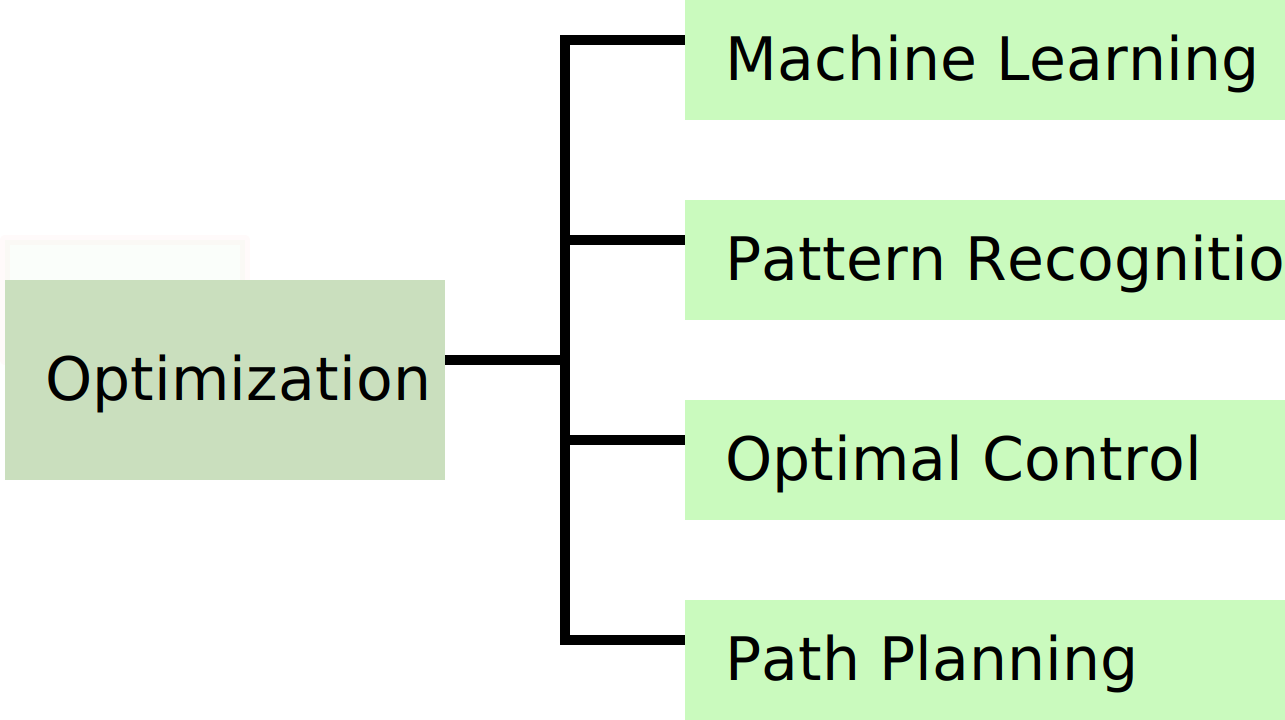
\includegraphics[width = .8\textwidth]{./figure/optimization}
\end{figure}
\end{frame}

\begin{frame}{Discrete Optimization}{Problem Definition}
\begin{block}{Objective}
\begin{equation}
\nonumber
f( \mathbf{X} ) = \sum_{ x_{i} \in \mathbf{X} } f(x_{i})
\end{equation}
\end{block}

\begin{block}{}
Combinatorial optimization
\begin{equation}
\nonumber
f(x_{1} , \cdots , x_{N} )= f(x_{1}) + \cdots + f(x_{N})
\end{equation}
\end{block}
\end{frame}


